\begin{multicols}{2}

\cappar

En este número os damos la solución al desafío del anterior número y os dejamos un nuevo desafío basado en un programa de televisión americano y una nueva partida. Al final os dejamos un recortable para que compartan con los mas pequeños. ¡Disfrútenlo!


\section*{El problema de Monty Hall}
¿Conoces el problema de Monty Hall? Es un desafío mental que debe su nombre al show de televisión \textit{Let's make a deal (Hagamos un trato)}, cuyo presentador era precisamente Monty Hall. Allí se presentaba el reto que os explicamos aquí.

Un concursante debe elegir una de las tres puertas que tiene delante, una de ellas esconde un premio (un coche) y las otras dos una cabra. Tras una primera elección, el presentador (que sabe dónde está el premio) abre una puerta que el concursante no haya elegido y que esconda una cabra. Tras eliminar esta puerta, le ofrece al concursante cambiar su elección.

\begin{figurebox}
  \centering 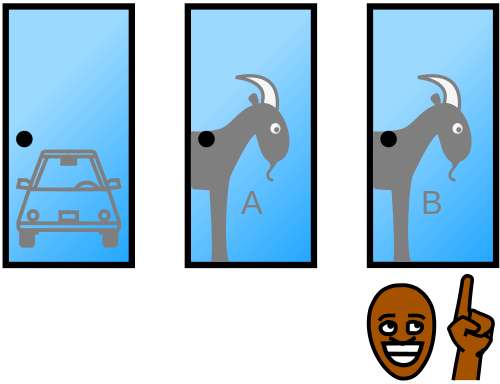
\includegraphics[scale=0.25]{500px-Monty-CurlyPicksGoatB.png}

  Figura 1: Elección de la puerta.
\end{figurebox}


La pregunta es ¿qué debería hacer el concursante, cambiar o quedarse con su puerta?

\subsubsection*{\textcolor{blue}{Respuesta}}
Este desafío se hizo famoso por ser extremadamente simple, pero con una respuesta sorprendente. Podríamos pensar que las dos puertas restantes tienen la misma probabilidad de esconcer el premio, pero no es así:

\begin{mybox}
  \begin{itemize}[leftmargin=0.2cm]
    \item Si el concursante cambia, tiene $2/3$ de probabilidad de ganar el premio (casi un $67\%$).
    \item Si se queda con su puerta, tiene $1/3$  de probabilidad de ganar el premio (cerca del $33\%$).
  \end{itemize}
\end{mybox}
La explicación es bien sencilla. Cuando eliges una puerta, tienes $1/3$ de probabilidad de acertar, y por lo tanto, tienes $2/3$ de probabilidades de haber fallado (evidentemente, esta probabilidad se reparte entre las dos puertas que no se han elegido, cada una con $1/3$).

Cuando el presentador abre una de las puertas malas, tu probabilidad de haber acertado no cambia en absoluto, sigue siendo $1/3$. Por lo tanto, tampoco cambia la probabilidad de que hayas fallado, que sigue siendo $2/3$. La diferencia es que ahora la probabilidad de haber fallado no se reparte entre tres puertas sino dos, pues el presentador ha abierto una de ellas.

Por lo tanto, tenemos dos puertas. El premio está en la tuya con probabilidad $1/3$ y debe estar en la otra con probabilidad $2/3$, de modo que lo más recomendable sería cambiar de puerta.


\section{El desafío: Monty Hall extendido}
Vamos a proponerte que resuelvas una variante del problema anterior, que bien podría ser útil para los concursantes de algunos programas de televisión.

Esta vez, vamos a suponer que tenemos \textbf{cuatro} puertas, una de las cuales esconde un premio que quieres ganar. Esta vez, cuando eliges por primera vez, el presentador te abre dos puertas malas y te da a elegir entre tu puerta y la que queda sin abrir.

La pregunta es, ¿qué probabilidades tienes de ganar si te quedas con tu puerta? ¿Y si cambias? ¡Esperamos vuestras respuestas!


\section{Ajedrez}

Te ofrecemos un reto ajedrecístico. En esta famosa partida, que te desvelaremos en el siguiente número, las blancas juegan y ganan. ¿Podrías encontrar la espectacular jugada ganadora?

\newgame
\mainline{1. e4 e5 2. d4 exd4 3. c3 dxc3 4. Nxc3 Bb4 5. Bc4 Qe7 6. Ne2 Nf6 7. O-O O-O 8. Bg5 Qe5 9. Bxf6 Qxf6 10. Nd5 Qd6 11. e5 Qc5 12. Rc1 Qa5 13. a3 Bxa3 14. bxa3 c6 15. Ne7 Kh8 16. Qd6 Qd8 17. Nd4 b6 18. Rc3 c5 19. Ndf5 Ba6}
% 20. Qg6}
\begin{center}
\showboard 
\end{center}

{\bf Las soluciones en el próximo número.}
\section*{\textcolor{redsol}{Soluciones del número anterior}}
\subsection*{El desafío: el borrón}
Para que sea múltiplo de 72 tiene que ser múltiplo de 8 y de 9
porque son coprimos. Para que sea divisible por 8, las tres últimas
cifras (79Y) tienen que formar un número múltiplo de 8. Luego,
tiene que ser 792. Por otro lado, para que sea múltiplo de 9, la
suma de sus dígitos tiene que ser múltiplo de 9: luego, X + 6 + 7
+ 9 + 2 = X + 24 tiene que ser múltiplo de 9. Conclusión, X = 3. El
número en cuestión era 36.792. Por lo tanto, cada televisor salió
a  511 (ya que multiplicado por 72 resulta ser 36.792).
\end{multicols}

Finalmente, os dejamos un recortable del juego chino Tangram para que lo compartan con los mas pequeños y algunas de las figuras a conseguir. 
\vspace{-0.3cm}
\begin{center}
\huge{\textcolor{bluesol}{Tangram}}


\includegraphics [scale=0.2]{Tangram.jpg} 
\includegraphics[scale=0.6]{tan7.jpg}
\end{center}

\newpage

%%% Local Variables:
%%% mode: latex
%%% TeX-master: "jugando"
%%% End:



